\documentclass[twocolumn]{revtex4}
\usepackage{graphics,graphicx,epsfig,amsmath,multirow,gensymb,commath,textcomp,natbib,blindtext,mhchem,tabularx,array,makecell,threeparttable,amssymb,relsize,csquotes}
\usepackage{listings}
\usepackage[a4paper, left=1.85cm, right=1.85cm, top=1.85cm, bottom=1.85cm]{geometry}   
\usepackage[normalem]{ulem}
\newcommand{\squeezeup}{\vspace{-2.5mm}}

\usepackage{lipsum}

\def\bibsection{\section*{\refname}} 
\renewcommand{\thesubsection}{\alph{subsection}}

\renewcommand\theadalign{bc}
\renewcommand\theadfont{\bfseries}
\renewcommand\theadgape{\Gape[4pt]}
\renewcommand\cellgape{\Gape[4pt]}

\begin{document}

\textheight=26.385cm
%Change textheight as the last resort...

\title{Constraining the geometry of the Universe using Type Ia supernovae and statistical methods}
 
\author{Jacky Cao, Group C3, Physics Problem Solving \\ Date of report: 28/02/2018}

\begin{abstract}              
Type Ia supernovae have the unique trait of being standard candles, their light curves can be used in cosmology to calculate and constrain cosmological parameters. In observing Type Ia supernovae and fitting model light curves to such data one can attempt to derive such values. We have monitored, collected, and analysed data for supernova explosions over a period of 34 days. A $16''$ and a $0.5$ m telescope situated in Durham and La Palma was used for this project. After calculating the magnitudes for a Type Ia (2017hhz) and Type Ia-91bg (2017hle) supernova object, we fitted template light curves with the Python program, \textit{SNooPy}. The quality of fit for the program's \texttt{fit()} function was deemed to be acceptable in accordance to the average reduced $\chi^2$ values calculated for the B and V photometric bands, $\chi^2_{\nu,B} \approx 1.38$ and $\chi^2_{V,\nu} \approx 2.95$ - a good fit requiring $\chi^2_{\nu} \approx1$. The distance modulus to the supernova 2017hhz was calculated by SNooPy to be $36.121\pm0.106$ mag, using this value we were able to compute $H_0=70\pm20$ km s$^{-1}$ Mpc$^{-1}$. However, the quoted error negates the meaning of $H_0$ as it is too large of an uncertainty. In improving the accuracy and uncertainties we suggest that more observations of the supernovae were required, and constraining values should be used for the parameters in SNooPy's templates.
\end{abstract}

\maketitle

\vspace{-3ex}
\section{Introduction and Theory} 
\vspace{-2ex}
In cosmology, one can argue that one of the most important observable events are supernova explosions. As a massive main sequence star runs out of nuclear fuel to burn, the equilibrium configurations which initially provided structure will cease to exist. What follows is a cataclysmic supernova explosion \cite{longair}. 

We can generally class supernova explosions into two separate groups, Type I and Type II supernovae. The main distinction arises due to the fact that Type I's have an optical spectra which contains no Balmer hydrogen features, whilst Type II supernovae do contain this hydrogen feature \cite{mod_ast}. 

Within these two subclasses there are further divisions which can be characterised through their spectra and through features as found in their light curves \cite{obs_phys_class_sn}. Light curves are a way to show the evolution of a supernova's magnitude as time passes. For example, with two of the subclasses of Type II supernovae, Type II-L and Type II-P, they can be classed from features of their light curves. For a Type II-L supernova there is a rapid linear decrease in magnitude, and with a Type II-P we see a constant magnitude after maximum \cite{mod_ast}.

For the application of supernovae in cosmology, we must turn to the variety of Type Ia.

\vspace{-3ex}
\subsection{Type Ia Supernovae}
\vspace{-2ex}
It is accepted that the light curves of Type Ia supernovae are generally homogeneous \cite{posn}, this means that they can be utilised as standard candles therefore allowing us a measure of cosmic distance. 

Their homogeneity arises due to the mechanism behind the explosion. The progenitor system for Type Ia's consist of a binary system with a primary white dwarf and secondary star which has a mass close towards the Chandrasekhar limit of $1.4 M_{\odot}$ \cite{mod_ast, posn}. The white dwarf will accrete matter from it's companion until it itself reaches the critical mass limit. After this point we would then expect the primary star to collapse into a neutron star, however this is not what happens. Instead, we find that a supernova explosion occurs. An event which arises due to a massive disruption to the star's internal structure by a large amount of energy. [[give a rough value]]

It is currently understood that as the white dwarf accretes matter it heats up and produces thermonuclear energy. This energy is achieved in the stellar interior at a temperature of $10^9$ K, as a result a disruption to the electron degeneracy pressure takes place. The star becomes gravitationally unstable from the nuclear energy and a total collapse into a neutron star is prevented \cite{longair, posn}.

This particular mechanism can be used to explain the standard profile of Type Ia light curves. Using these plots, the maximum B band photometric magnitude can be obtained with the following equation,
\begin{equation}
M_{\max}(B)=-21.726+2.698\Delta m_{15}(B),
\end{equation}

where $\Delta m_{15}(B)$ is the decline rate parameter or Phillips' parameter \cite{high_en_astro}. This is defined as the mean rate of decline of the B band light curve from peak light to 15 days after the maximum \cite{abs_phil}. This parameter relates the apparent magnitude to time and provides a way to compare and contrast different Type Ia supernovae. 

With values for the absolute magnitude of Type Ia supernovae and with values of their redshift obtained from spectroscopic observations, the distance to these objects can then be calculated using the following equation, 
\begin{equation}
\mu = 5 \log_{10}(d) - 5,
\end{equation}

where $\mu$ is the distance modulus and can be defined as the absolute magnitude of supernova subtracted from it's apparent magnitude, and we define $d$ is the distance to the supernova in parsecs \cite{mod_ast}. 

From data sets of Type Ia supernovae we can easily employ them to calculate the geometry of the universe. But before that, we must first understand what cosmological parameters are and how they can be constrained.

\vspace{-3ex}
\subsection{Cosmological Parameters}
\vspace{-2ex}
At large cosmological distances, the appearance of objects will be affected by the spacetime which it travels through. If we therefore wanted to describe the geometrical properties of the universe, we would require to solve Einstein's general theory of relativity. From \textit{An Introduction to Modern Astrophysics} \cite{mod_ast} we can build the framework required to calculate and compute cosmological parameters. 

If we solve Einstein's field equations for an isotropic, homogenous universe a description of the evolution of the universe can be obtained in the form of a differential equation which is also known as the Friedmann equation. In the 1922 form of the equation, a non-static universe is accounted for,
\begin{equation}
\Big[ \Big( \frac{1}{R} \frac{dR}{dt} \Big)^2 - \frac{8}{3} \pi G \rho \Big] R^2 = -k c^2,
\label{eqn:1922_friedmann}
\end{equation}

where $R(t)$ is the scale factor, $G$ the gravitational constant, $\rho$ is the mass density, $k$ is a parameter which describes the shape of the universe, and $c$ is the speed of light in a vacuum.

$k$ can be defined as a constant which is equal to $-1$ for a negatively curved universe, $0$ for a spatially flat universe, and $+1$ for a positively curved universe \cite{longair}. 

Separate work performed by Einstein eventually led to a cosmological constant $\Lambda$ being introduced in the Friedmann equation. This was included in the form of $\tfrac{1}{3}\Lambda c^2$ within the square brackets of the left hand side of Equation \ref{eqn:1922_friedmann}. Whilst Einstein included this term to account for his static and closed universe, as a consequence of observations which implied an accelerating universe, astronomers in the 1990s eventually related the cosmological constant to dark energy.

Taking the Friedmann equation, it can be rewritten so that it considers a three component universe composed of baryonic and dark matter, relativistic photons and neutrinos, and dark energy, 
\begin{equation}
\Big[ \Big( \frac{1}{R} \frac{dR}{dt} \Big)^2 - \frac{8}{3} \pi G (\rho_{M} + \rho_{\text{rel}} + \rho_{\Lambda} )\Big] R^2 = -kc^2,
\end{equation}

where $\rho_{M}$ is the density of matter, $\rho_{\text{rel}}$ is the density of the radiation, and $\rho_{\Lambda}$ is the density of the dark energy. Combining these densities with a critical density we can adapt the Friedmann equation so that it includes \textit{cosmological parameters}, these are values which describe the content makeup of the universe in terms of matter and energy. This critical density is defined as the value of the density that will result in a flat ($k=0$) universe. We see that the Friedmann equation becomes,
\begin{equation}
H^2 [1-(\Omega_{M} + \Omega_{\text{rel}} + \Omega_{\Lambda})]R^2 = -kc^2,
\label{eqn:friedmann_old}
\end{equation}

where $H$ is the Hubble parameter and is related to the scale factor and expansion factors of the universe, $\Omega_{M}$ is the matter density parameter, $\Omega_{\text{rel}}$ is density contribution from radiation, and $\Omega_{\Lambda}$ is defined as the dark energy density parameter.

With this in hand, it is now possible to calculate the proportions of the universe which amounts to matter and the amount which is energy. In these calculations, cosmologists normally choose to omit the contribution from radiation as it is a negligible amount. Results from the Wilkinson Microwave Anisotropy Probe (WMAP) show that $\Omega_{\text{rad}}=8.25 \times 10^{-5}$, an insignificant value when compared to $\Omega_{\Lambda}=0.74 \pm 0.04$ and $\Omega_{M} = 0.27 \pm 0.04$ \cite{mod_ast}. 

Using these cosmological variables we can additionally define the total density parameter,
\begin{equation}
\Omega \equiv \Omega_{M} + \Omega_{\Lambda} + (\Omega_{\text{rel}}).
\label{eqn:total_density}
\end{equation}

Inputting the WMAP data into Equation \ref{eqn:total_density} we see that a value of $\Omega \sim 1$ is produced, indicating that the universe is flat with $k=0$ and that dark energy is the dominant factor in the expansion of the universe \cite{mod_ast}.

This result was obtained through measurements of the cosmic microwave background, however it would be especially useful if data from other cosmic objects could be used. We therefore return to Type Ia supernovae as they are the perfect candidate to help us constrain the geometry of the universe. They are more readily accessible and observations can be more easily made. 

\vspace{-3ex}
\subsection{Cosmological Parameters from Type Ia Supernovae}
\vspace{-2ex}
To constrain the cosmological parameters using supernovae we do not look at the Friedmann equation directly. Instead, the main methodology is to use a Least Squares test to select the best model which would then correspond to cosmological parameters. We can define this test as the $\chi^2$ statistic, 
\begin{equation}
\chi^2 = \sum \frac{(f_\text{obs}-f_\text{model})^2}{\sigma_\text{obs}^2},
\label{eqn:chi_eqn}
\end{equation}

where $f_\text{obs}$ is the peak observed flux of the supernova, $f_\text{model}$ is the model flux for the supernova calculated using the corresponding redshift and with certain defined cosmological parameters, and $\sigma_\text{model}$ is the uncertainty on the observational flux \cite{script}.

Obtaining $f_\text{obs}$ is a simple matter, we can find it by using a rearranged form of,
\begin{equation}
m_\text{obs}=m_0 - 2.5\log_{10}(f_\text{obs}),
\end{equation}

that is, $m_\text{obs}$ is the effective peak magnitude of the supernova, $m_0$ is a constant with a value of $-20.45$, and $f$ is the supernova flux in units of erg cm$^{-2}$s$^{-1}$\AA$^{-1}$ \cite{script}.

On the other hand, to find $f_\text{model}$ we begin by defining the flux equation for a certain model,
\begin{equation}
f_\text{model}=\frac{L_\text{peak}}{4\pi [R_0 S(\eta)]^2 (1+z)^2},
\label{eqn:fmodel}
\end{equation}

where $L_\text{peak}$ is the peak luminosity value for Type Ia supernovae, $R_0 S(\eta)$ is the comoving distance between the observer and where the supernova exploded in space, and $z$ is the redshift for the supernova \cite{script}.

To find $L_\text{peak}$, the low-redshift ($z<0.1$) Type Ia supernovae objects can be selected out of a data set and then Equation \ref{eqn:fmodel} can be used by taking the approximation $R_0 S(\eta) \approx cz/H_0$. Optimum $L_\text{peak}$ can then found by using Equation \ref{eqn:chi_eqn}, the smallest value for $\chi^2$ corresponds to the best luminosity. This value can then be applied to calculations involving supernovae which have redshifts higher than 0.1. For this data set the comoving distance cannot be simply approximated so we must use the following definition,
\begin{equation}
R_0 \eta = c \int_0^z \frac{dz'}{H(z')},
\label{eqn:comoving_integral}
\end{equation}

we find that within this integral we need to integrate a form of the Friedmann equation between a value for the redshift of the supernova $z$ and no redshift. We can derive this by using Equation \ref{eqn:friedmann_old} and with the assumption that if the universe is flat then $\Omega_{M} = 1 - \Omega_{\Lambda}$, reducing the cosmological parameters which we have to find \cite{script}. 

We now arrive at the following result for the Hubble Parameter,
\begin{equation}
H^2 = H_0^2 [(1+z)^3 - \Omega_{\Lambda} ((1+z)^3-1)],
\label{eqn:hubble_parameter}
\end{equation}

where $H_0$ is a value for the Hubble's constant, $z$ is the redshift for a supernova, and $\Omega_\Lambda$ is a cosmological constant.

To find the optimum value for $\Omega_\Lambda$ we can select a range from 0.0 to 1.0 and then calculate $f_\text{model}$ and $\chi^2$ for each number. Identical to finding $L_\text{peak}$, the best value for the cosmological parameter is found by choosing the minimum value for $\chi^2$. Through the usage of this least squares method one is able to explore cosmological parameters using Type Ia supernova data sets.

\vspace{-4ex}
\subsection{Project Aims}
\vspace{-2ex}
In this paper we discuss the experimental work performed to constrain cosmological parameters using Type Ia supernova data. Least Squares and Bayesian methods are initially explored, then details of experiments involving models which contain more than two parameters are analysed.

\vspace{-3ex}
\section{Results and Discussion} 
\label{sec:results_discussion}
\vspace{-3ex}
\subsection{$\chi^2$ Statistics} 
\vspace{-2ex}
To calculate cosmological parameters using supernovae we must first obtain data sets of Type Ia supernovae which contain redshift, effective magnitude and the uncertainty on that magnitude. We specify effective magnitude as this means that it has been correct for light curve stretching and galactic dust extinction amongst other factors \cite{script}. This means that the magnitudes used in our calculations will be more accurate and thus produce more accurate parameters. 

In our first experiments we chose to use a data of set of 42 high-redshift ($z>0.1$) Type Ia supernovae from the Supernova Cosmology Project and 18 low-redshift ($z<0.1$) ones from the Cal\'{a}n Tololo Survey \cite{dataset_1}. As indicated in our previous discussion of the experimental theory we require the low-redshift supernovae to `calibrate' the Type Ia data so that Equation \ref{eqn:fmodel} can be used. In doing so we find $L_{\text{peak}} = (3.1\pm0.1) \times 10^{35}$ W for the peak luminosity and in using this we can then proceed to calculate $\Omega_\Lambda$.



\begin{table}[h!]
\centering
\begin{tabular}{c@{\hskip 15pt}c@{\hskip 15pt}c@{\hskip 15pt}c} 
 \hline
 \textbf{Parameter} & \textbf{$\boldsymbol{\chi^2}$} & \textbf{MCMC} & \textbf{Literature} \\ [0.5ex] 
 $L_{\text{peak}}$ ($\times 10^{35}$ W) & $3.1\pm0.1$ & $3.4\pm0.1$ & 1\\
 $\Omega_\Lambda$ & 18.8 & 0.2 & 1 \\
 $\Omega_k$ & - & 1 & 1 \\
 $\Omega_M$ & - & 1 & 1 \\
 $\Omega_\text{rad}$ & - & 1 & 1 \\
 $w$ & - & 1 & 1\\
 \hline
\end{tabular}
\caption{10 days worth of data was analysed to produce magnitudes and their uncertainties for the B and V photometric bands for Type Ia supernova, 2017hhz. }
\vspace{-0.5em}
\label{table:2017hhz_data}
\end{table}

aassa

\begin{figure}[!h]
\begin{center}
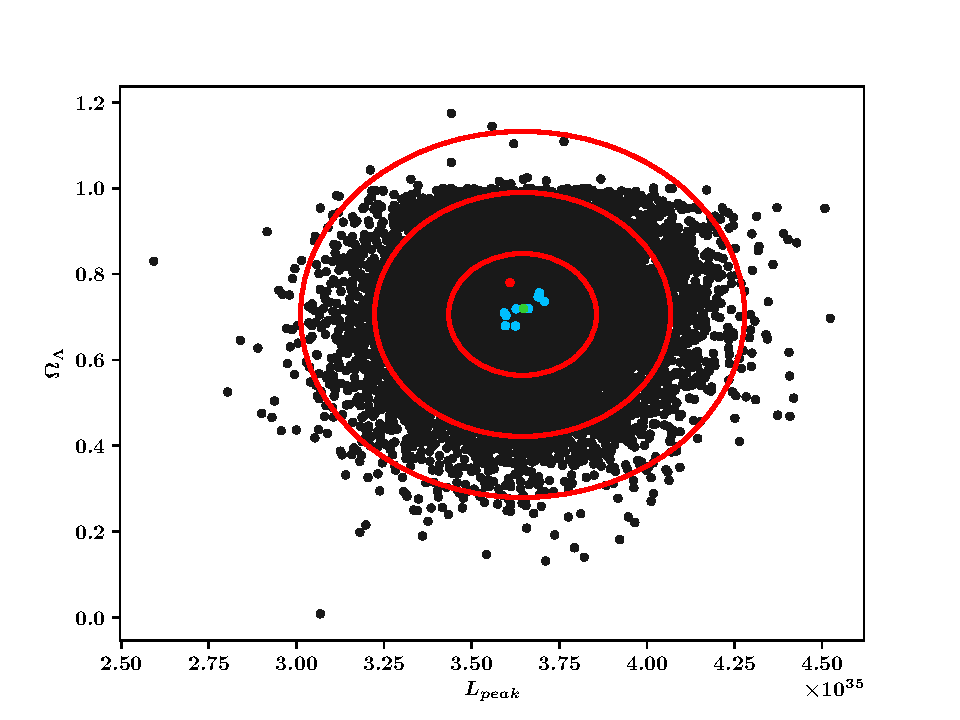
\includegraphics[width=9.25cm]{results/ol_lp_complete}
\caption[]{Plot showing the general forms of Type Ia supernovae in the B and V bands. Archival data was translated along the time and magnitude axes to produce the general forms of the light curves. The B band has been offset by a magnitude of $3$ to allow us to see both graphs clearly. The supernovae which were used to plot this graph are: \em{1994ae, 1994S, 1995bd, 1996bo, }\em  and \em{1998aq }\em \cite{jha, matheson}. }
\vspace{-3ex}
\label{fig:ol_lp_complete}
\end{center}
\end{figure}

asdasd

\vspace{-3ex}
\subsection{Bayesian Statistics} 
\vspace{-2ex}

asdasd


\begin{figure}[!h]
\begin{center}
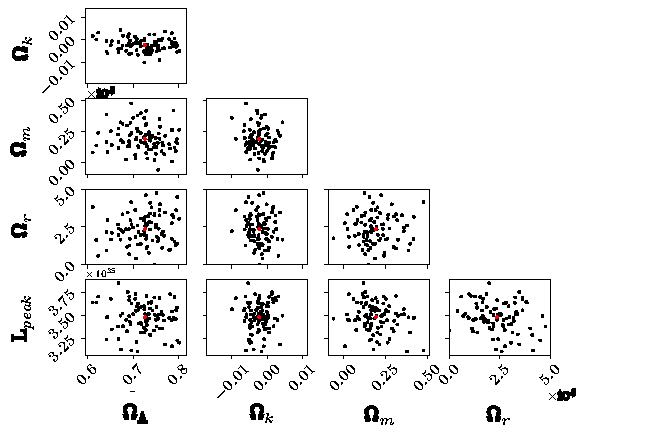
\includegraphics[width=9.25cm]{results/triangle}
\caption[]{Plot showing the general forms of Type Ia supernovae in the B and V bands. Archival data was translated along the time and magnitude axes to produce the general forms of the light curves. The B band has been offset by a magnitude of $3$ to allow us to see both graphs clearly. The supernovae which were used to plot this graph are: \em{1994ae, 1994S, 1995bd, 1996bo, }\em  and \em{1998aq }\em \cite{jha, matheson}. }
\vspace{-3ex}
\label{fig:triangle}
\end{center}
\end{figure}


sdfasdfsdfsad

\vspace{-3ex}
\subsection{Further Investigation} 
\vspace{-2ex}

asdasd

\vspace{-5ex}
\section{Conclusions}
\vspace{-2ex}

In conclusion, we have found that it is possible to constrain cosmological parameters of the universe using Type Ia supernova data.

\vspace{-3ex}
\bibliographystyle{abbrv}
\bibliography{supernova_cosmology}

\clearpage
\appendix

\vfill
\twocolumngrid
\vspace{-3ex}
\section{??}
\vspace{-2ex}



\clearpage
\end{document}